\subsection{Neural Network Architectures}
\label{sec:nn-architectures}

To systematically study the trade-off between network size and verifiability, we constructed a family of convolutional neural network (CNN) models designed specifically for image classification tasks with grayscale inputs of size $28 \times 28$ pixels. Each model outputs one of three possible classes.

All networks share a consistent two-layer convolutional architecture followed by a compact fully connected head, as illustrated in Figure~\ref{fig:cnn-arch}. The convolutional layers employ $3 \times 3$ kernels, a stride of 2, and padding of 1, sequentially reducing the spatial dimensions from $28 \times 28$ to $7 \times 7$. The output of the convolutional backbone is flattened and passed through a fully connected layer with a fixed hidden size of 4, or 3 in the case of Model~239, before the final classification layer producing 3 output logits.



\begin{figure}[ht]
\centering
\begin{tikzpicture}
    \node at (0,0) {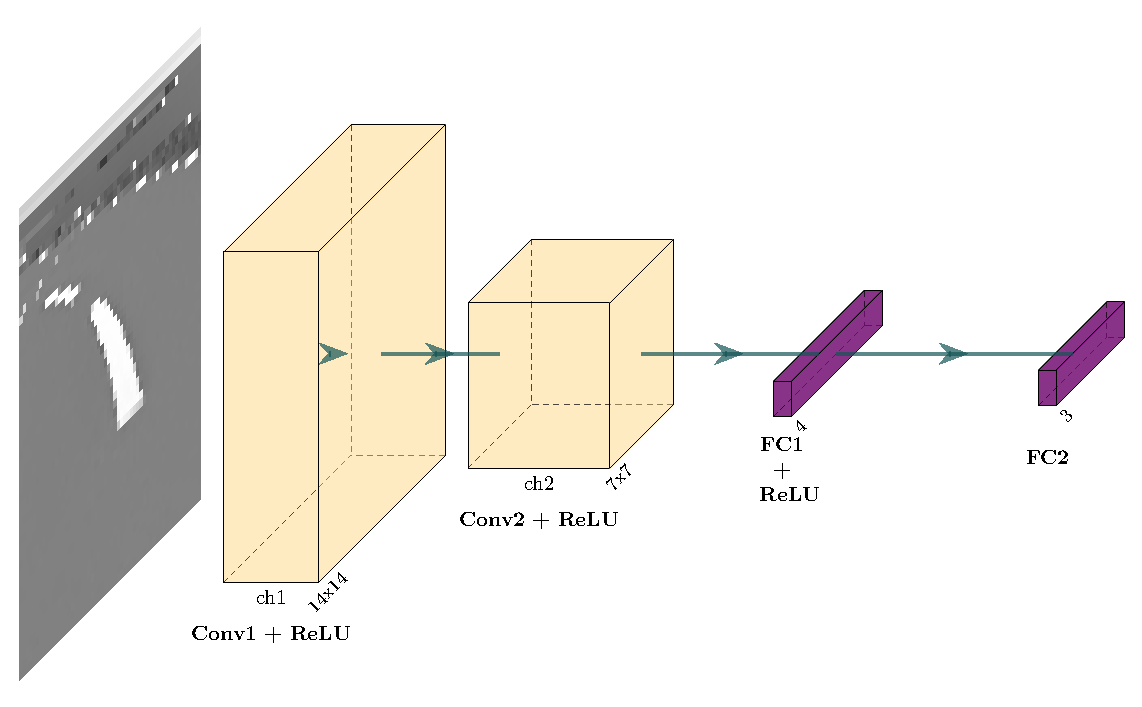
\includegraphics[width=\textwidth]{figures/test_simple.pdf}};

\end{tikzpicture}
\caption{The common CNN architecture used for all models. It consists of two convolutional layers followed by two fully connected layers. The number of channels in the convolutional layers ($ch_1, ch_2$) varies across models as detailed in Table~\ref{tab:model-params}.}
\label{fig:cnn-arch}
\end{figure}

The specific hyperparameter configurations for the different model sizes used in our study are detailed in Table~\ref{tab:model-params}.

\begin{table}[htbp]
\centering
\caption{Model parameter configurations. The number of channels in the first ($ch_1$) and second ($ch_2$) convolutional layers are varied to achieve different total parameter counts.}
\label{tab:model-params}
\begin{tabular}{l c c r}
\toprule
\textbf{Model} & \textbf{$ch_1$} & \textbf{$ch_2$} & \textbf{Total Parameters} \\
\midrule
239    & 4  & 1  & 239 \\
1k    & 4  & 4  & 991 \\
5k  & 10 & 17  & 4,998 \\
20k   & 37 & 37 & 19,999 \\
\bottomrule
\end{tabular}
\end{table}


